\chapter{Evaluation}
\label{sec:eval}

\section{Simulation Model} 

%%%%%%%%%%%%%%%%%%%%%%%%%%%%%%%%%%%%%%%%%%%%%%%%%%%%%%%%%%%%%%%%%%%%%%
\begin{figure*}[h!]
\centering
     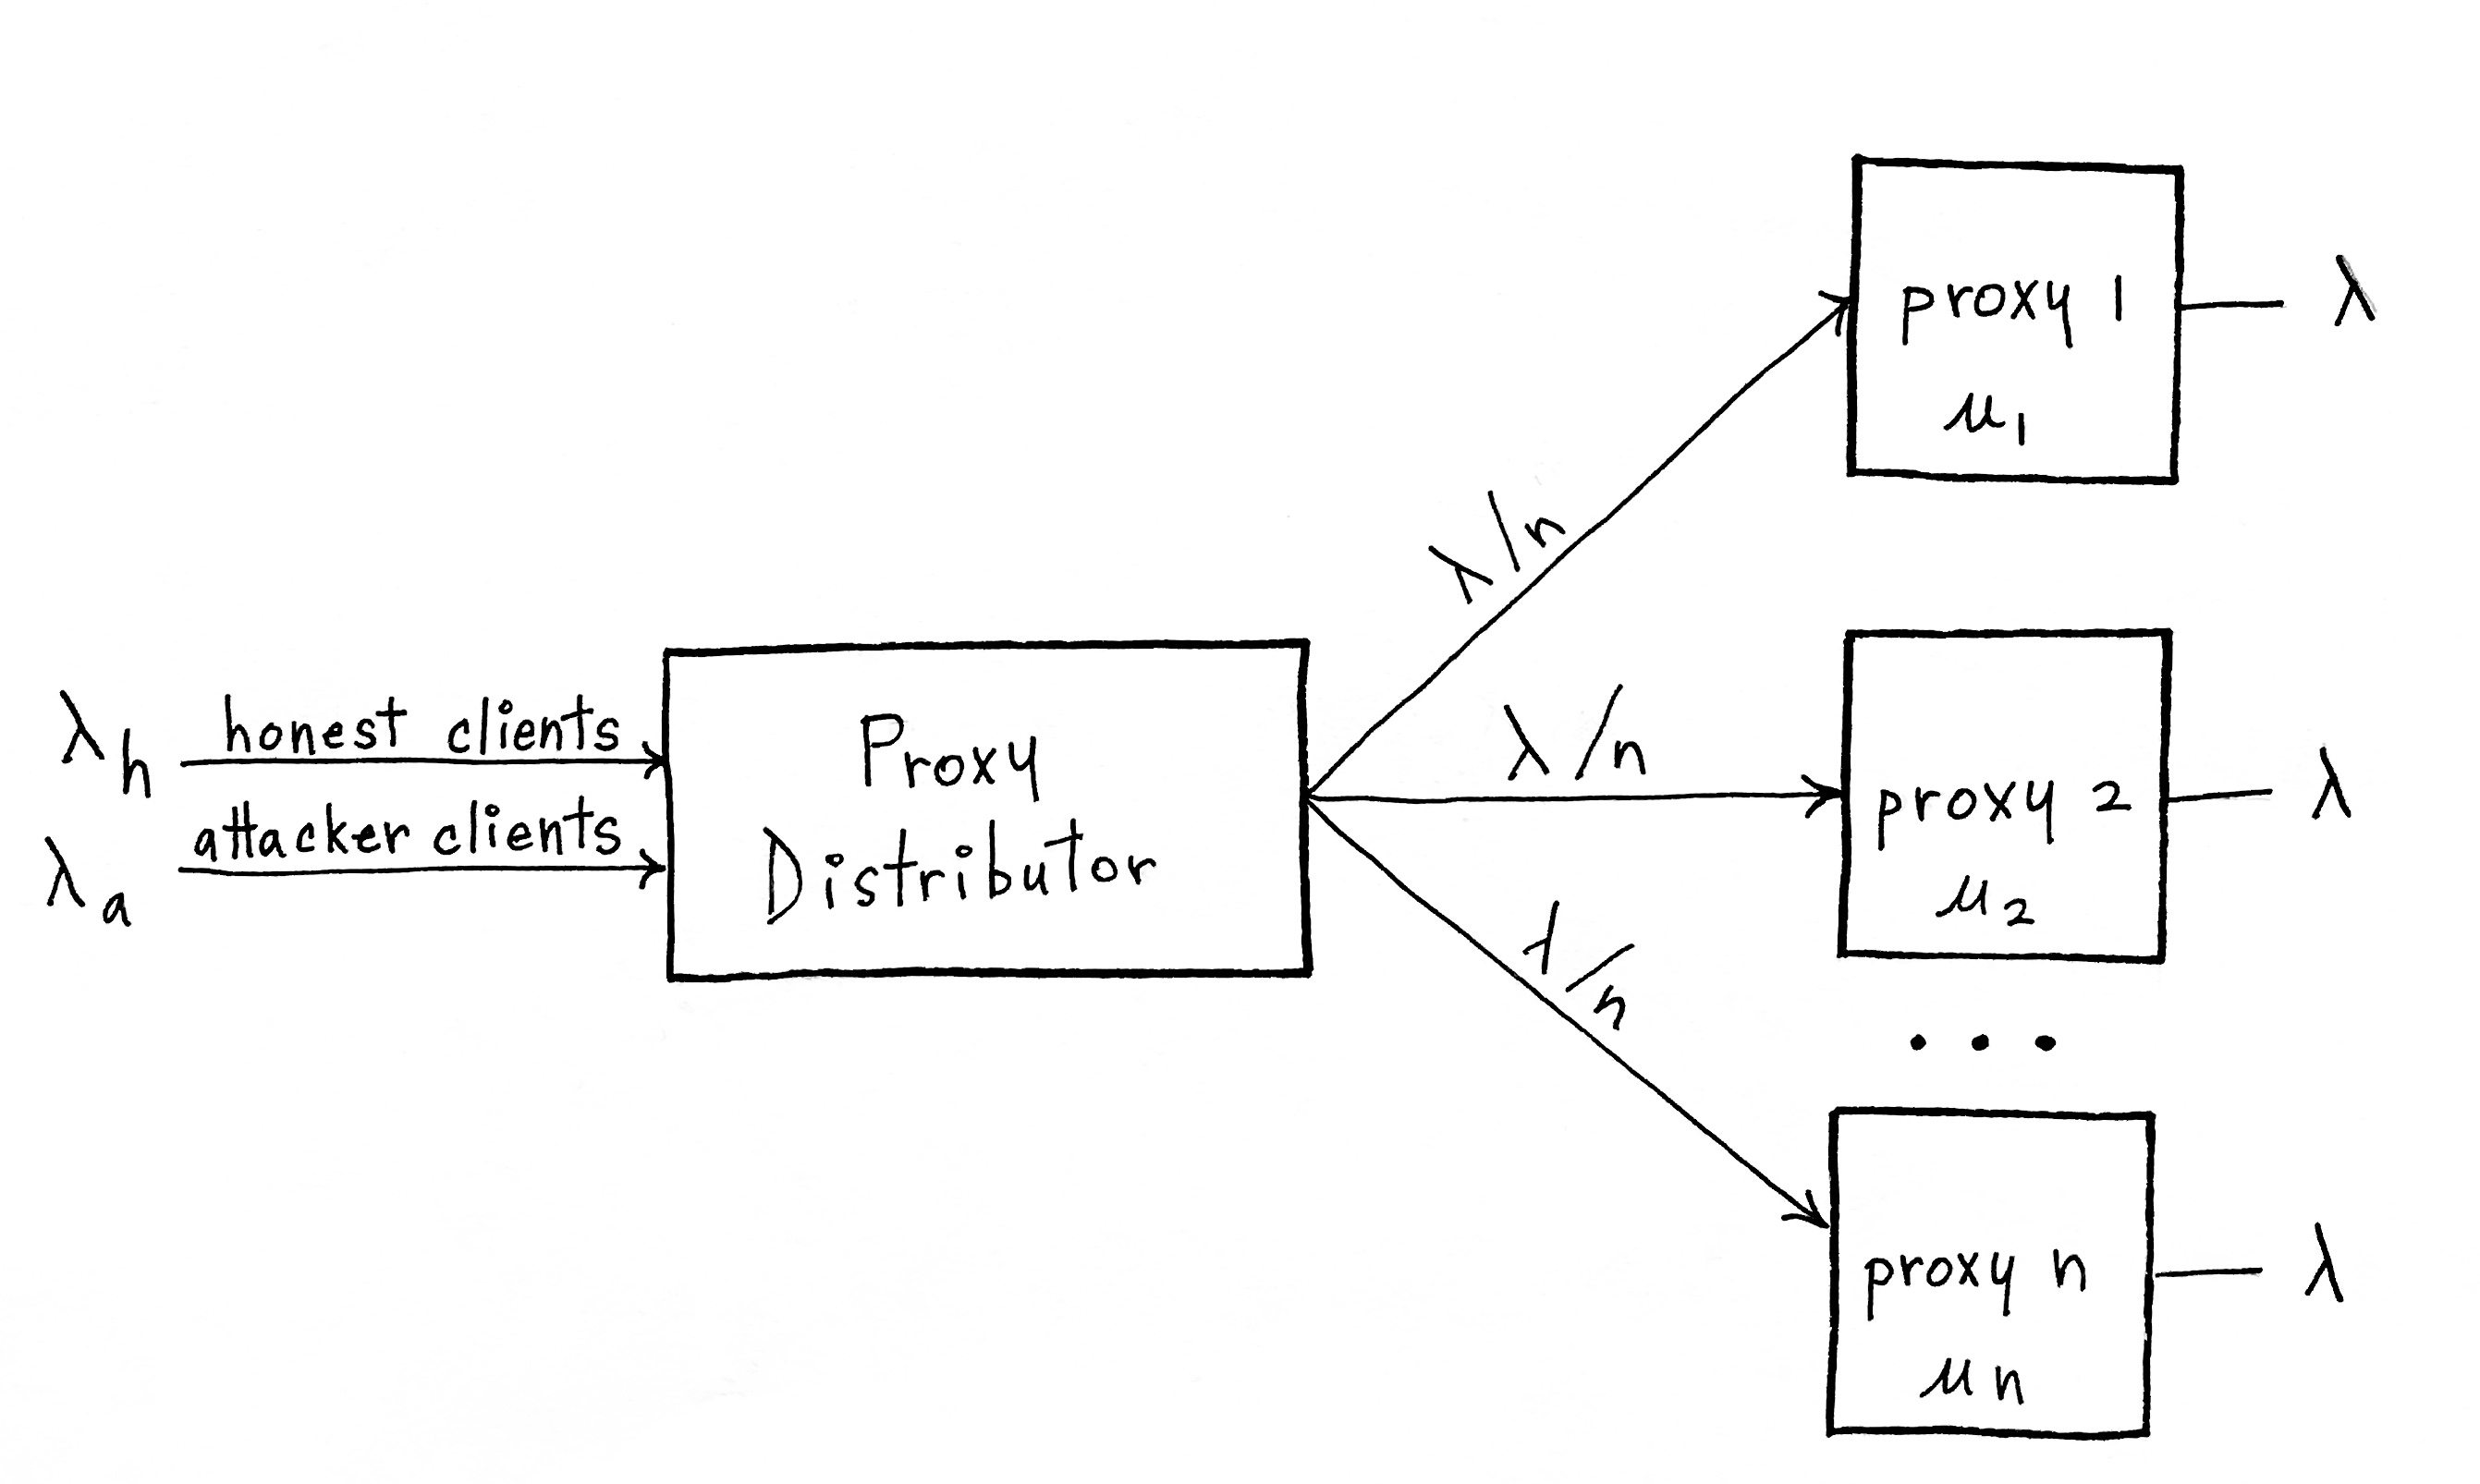
\includegraphics[width=1.0\textwidth]{fig/mmck_queue.png}
    \caption{M/M/c/k with uniform random distribution}

    \label{fig:mmck}
\end{figure*}
%%%%%%%%%%%%%%%%%%%%%%%%%%%%%%%%%%%%%%%%%%%%%%%%%%%%%%%%%%%%%%%%%%%%%%

Before considering details of the simulation experiments, we formalize the simulation model and how it applies to the needle algorithm proxy distribution strategy. The notion of static and dynamic models stems from static and dynamic routing in networks. Mitzenmacher redefined static and dynamic models for task allocation and applied this to the balls and bins model \cite{mitzenmacher1996power}. In this context, a ball is a task and a bin is a processor. The primary distinguishing features of the static model is that there are a finite number of tasks that are assigned to processors and these tasks do not leave. The static system model completes its execution when all of the tasks are allocated. This model execution is generally represented in a bipartite graph. A static model applied to the proxy distribution problem assigns a finite number of clients to proxies in one round.

The dynamic model captures scenarios that are more realistic than what may be represented in the static model. For example, tasks in the dynamic model may enter and leave the system over time. In the open dynamic model, there may not be a fixed number of tasks. The closed dynamic model allows for tasks to enter and leave over time, but there is a fixed number of arrivals. A dynamic system does not have a final termination time as in the static model. The advantage of a dynamic model is that one can observe the behaviour of a system over time.

We are interested in how proxies are enumerated by a censor throughout the system's lifetime, so the open dynamic model suits our scenario well. Utilizing an open dynamic model allows us to observe trends and compare different approaches temporally. However, our clients don't \textit{leave} in the traditional sense; we assume that once a proxy is discovered, the knowledge of a proxy cannot leave or exit. 

\begin{table}[h]
  \centering
	\begin{tabular}{ll}
	\hline
	\cline{1-2}
	Parameter Name   & Description  \\
	\hline
    $\lambda_h $ client arrival rate & intensity of client arrival rate $1/\lambda$ \\
	$\lambda_a$ attacker arrival rate  & intensity of attacker client arrival rate $1/ \lambda$\\
	n     & number of proxies \\
	\hline
	\end{tabular}
  \caption{Variables in the Simulation}
  \label{tab:vars}
\end{table}

In addition to the dynamic model, the queue model is a standard that suits the problem of proxy distribution well. Mitzenmacher models the power of two choice algorithm as an idealized process, or a queue system of infinite size, that is later related to a finite system by bounding the error between the two \cite{mitzenmacher1996power}. 

Our simulation is best described as a feed-forward network of M/M/c/k queues. This is similar to a load balancing system with a constant number of servers. However, in this scenario, the load balancer is in fact the proxy distributor that is responsible for distributing clients to proxies. Figure \ref{fig:mmck} shows the network queue layout where the proxy distributor assigns clients to proxies uniform randomly, where the arrival of clients to proxies is evenly distributed $\lambda/n$. 

Clients arrive with a Poisson arrival distribution with variable $\lambda$ clients per minute. This means that, on average, one client appears at every $1 / \lambda$ minutes and we define this as the arrival intensity. In this model, we are additionally concerned with honest and malicious client arrival rates. As the proportion of attackers in the system increases, the arrival rate, or intensity of malicious client arrivals increases.

Each proxy has a service time that is exponentially distributed. This is not a traditional service rate because the system assumes short-lived client connections. The important function of the server is to keep a record of each client assignment that can be used by the censor to discover clients in the system. In other words, even if the client leaves the system, the censor still gains knowledge of the proxy and may impact the client's future connections to the known proxy, effectively mounting a potential future blocking attack on the proxy.

\textbf{Parameters.} Parameters in the simulation control the rate of honest and malicious client arrival intensity, the total number of proxies, and the size of the step for the needle algorithm. These are sweeping parameters; the simulation runs across a range of values for each parameter to produce a variety of conditions for the analysis. The analysis operates on the dependent variables such as maximum load and the expected time to overtake the system. The variable names and descriptions are outlined in table \ref{tab:vars}.

The simulator was written in Python using simpy, a discrete event based simulator.\footnote{https://simpy.readthedocs.io/en/latest/} The evaluation uses numpy\footnote{http://www.numpy.org/} and matplotlib\footnote{https://matplotlib.org/} for data manipulation and graphing.

\section{Enumeration Results}

%%%%%%%%%%%%%%%%%%%%%%%%%%%%%%%%%%%%%%%%%%%%%%%%%%%%%%%%%%%%%%%%%%%%%%
\begin{figure*}[h!]
\centering
     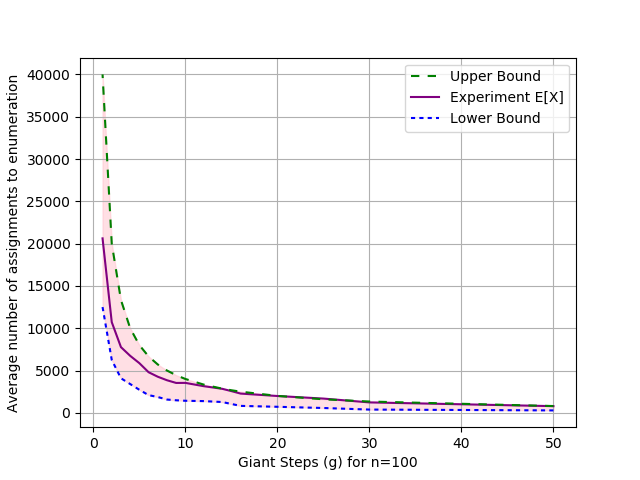
\includegraphics[width=0.8\textwidth]{fig/needle_expected_value_n_100.png}
    \caption{Giant step enumeration comparison for 100 proxies}

    \label{fig:gsn100}
\end{figure*}
%%%%%%%%%%%%%%%%%%%%%%%%%%%%%%%%%%%%%%%%%%%%%%%%%%%%%%%%%%%%%%%%%%%%%%

\textbf{Giant step analysis.} We ran the needle algorithm in the simulator, with only malicious attacker clients, to observe how many assignments a censor needs to enumerate all of the proxies. In section \ref{theorem:UBEX}, we analyzed the giant step version of the needle algorithm where step size $g > 1$. Results are shown in Figure \ref{fig:gsn100} for 1000 trials using 100 proxies in each experiment. The experimental results are shown in the black, solid line. The upper and lower bounds, $E[X] \leq \frac{(n^2)H_{\lceil{H_n}\rceil}}{g}$ and $E[X] \geq (g)(s^2H^{(2)}_{\lfloor{H_n}\rfloor})$ respectively, are shown in dashed lines.

Table \ref{tab:enumn100} shows the numerical data from these 1000 trials of varying step size for 100 proxies, and the calculated upper and lower bounds.

\begin{table}[t]
\centering
\begin{tabular}{l|l|l|l|l}
             Sublist (s) & Step (g) & Upper Bound & Experiment & Lower Bound  \\
\hline
\hline
100 & 1 & 40000 & \textbf{20619} & 12500 \\\hline
50 & 2 & 20000 & \textbf{10718}	& 6250 \\\hline
33 & 3 & 13333	& \textbf{7763} & 4083 \\\hline
25 & 4 & 10000 & \textbf{6738} & 3403 \\\hline
20 & 5 & 8000 & \textbf{5869} & 2722\\\hline
16 & 6 & 6667 & \textbf{4800} & 2091 \\\hline
12 & 8 & 5000 & \textbf{3850} & 1568\\\hline
10 & 10 & 4000	& \textbf{3537} & 1424\\\hline
8 & 14 & 2857 & \textbf{2839} & 1276\\\hline
5 & 20 & 2000 & \textbf{1987} & 712\\\hline
4 & 25 & 1600 & \textbf{1683} & 569\\\hline
2 & 50 & 800 & \textbf{788} & 285\\\hline
1 & 100 & 400 & \textbf{100} & 100\\\hline

\end{tabular}
\caption{Experimental results for 100 proxies over 1000 trials\label{tab:enumn100} }
\end{table}

\textbf{Enumeration Comparison.} We compare the four different algorithms in Figure \ref{fig:comparison}. The y-axis shows the average enumeration time over 1000 trials where a higher number of assignments is favourable because it takes longer for a censor to discover all of the proxies. The x-axis shows the trials over different sizes of $n$ proxies. We know from the Coupon Collector Problem \ac{CCP} that the uniform random distribution of coupons results in $nH_n$ total assignments before collection. We see that the uniform random distribution of Tor's \texttt{bridgedb} follows a similar enumeration. We use the regular power of 2 choices algorithm to show how a more optimal load balancing algorithm results in faster enumeration \cite{xu2011generalized}. In the upcoming section, we'll take a closer look at the load balancing properties of each of these algorithms.

%%%%%%%%%%%%%%%%%%%%%%%%%%%%%%%%%%%%%%%%%%%%%%%%%%%%%%%%%%%%%%%%%%%%%%
\begin{figure*}[h!]
\centering
     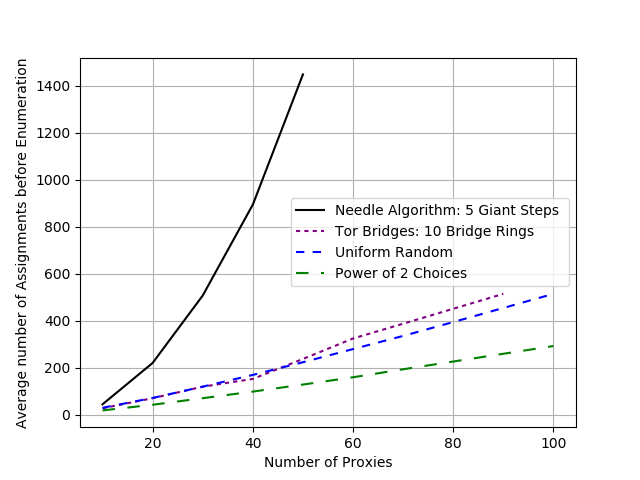
\includegraphics[width=0.8\textwidth]{fig/comparison_graph.png}
    \caption{Number of assignments before enumeration for each algorithm for n=10 to 100 proxies.}

    \label{fig:comparison}
\end{figure*}
%%%%%%%%%%%%%%%%%%%%%%%%%%%%%%%%%%%%%%%%%%%%%%%%%%%%%%%%%%%%%%%%%%%%%%

\section{Load Balancing Results}

Recall that in the analysis, Lemma $9$ in section $3.3$ stated that $px_{n/2}$ has the optimal load. In the experiments shown in Figure \ref{fig:needlelb2}, we ran the needle trials until all of the proxies were enumerated and then kept running the trials until twice the number of enumeration time. We see that the load balancing is divided into two halves centred around the optimal load. We also note that the maximum load for each of the experiments is no more than 4\% of the total load.

%%%%%%%%%%%%%%%%%%%%%%%%%%%%%%%%%%%%%%%%%%%%%%%%%%%%%%%%%%%%%%%%%%%%%%
\begin{figure*}[h!]
\centering
     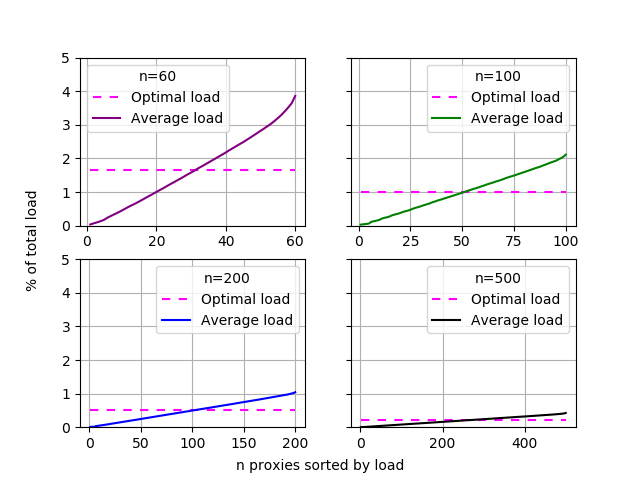
\includegraphics[width=1.0\textwidth]{fig/load_balance_needle_to_twice_enum_60_100_200_500.png}
    \caption{Needle Load Balancing until all proxies are enumerated twice for $n=60, 100, 200, 500$.}

    \label{fig:needlelb2}
\end{figure*}
%%%%%%%%%%%%%%%%%%%%%%%%%%%%%%%%%%%%%%%%%%%%%%%%%%%%%%%%%%%%%%%%%%%%%%

We wish to observe and compare the load balancing tendencies of each of the four algorithms. The x-axis in Figure \ref{fig:lbcomp} orders all of the proxies by their respective loads. The y-axis shows the percentage of the total load that each proxy holds. We ran each algorithm for 5000 assignments with a total of 100 proxies. 

A distinguishing feature of each algorithm is their varying degree of even distribution of assignments to proxies. The power of 2 choices algorithm gives the most evenly balanced distribution. The uniform random distribution results in the next best load balancing. Tor's mechanism is less balanced than uniform random but more balanced than the needle algorithm. The needle algorithm results in the worst load balancing.

%%%%%%%%%%%%%%%%%%%%%%%%%%%%%%%%%%%%%%%%%%%%%%%%%%%%%%%%%%%%%%%%%%%%%%
\begin{figure*}[h!]
\centering
     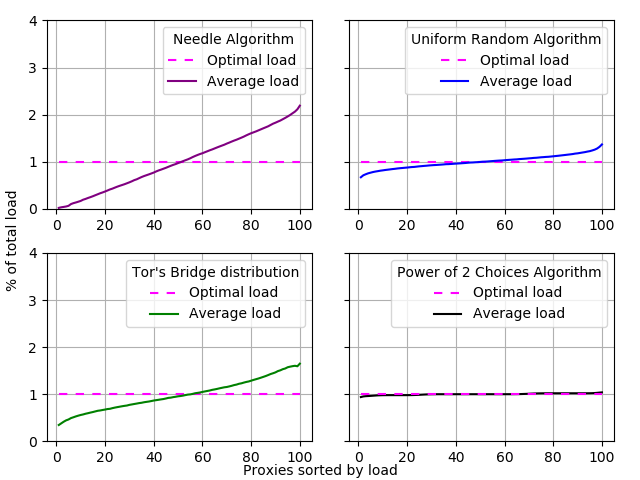
\includegraphics[width=1.0\textwidth]{fig/load_balance_comparison_to_5000_100.png}
    \caption{Load balancing results for each algorithm for n=10 to 100 proxies and 5000 assignments each.}

    \label{fig:lbcomp}
\end{figure*}
%%%%%%%%%%%%%%%%%%%%%%%%%%%%%%%%%%%%%%%%%%%%%%%%%%%%%%%%%%%%%%%%%%%%%%


\section{Bystander Results}
\label{sec:bystandereval}

Load balancing and the proportion of attackers directly affect the number of bystanders. Bystanders are those honest clients that still receive service in the presence of malicious clients. For the experiment in Figure \ref{fig:malcompare}, we run all of the algorithms so they each have 5000 assignments and the probability that a client is malicious is 50\%. We sort the proxies by their loads in increasing order and plot the numbers of malicious clients assigned to each proxy, from lowest loaded proxy to highest loaded.

%%%%%%%%%%%%%%%%%%%%%%%%%%%%%%%%%%%%%%%%%%%%%%%%%%%%%%%%%%%%%%%%%%%%%%
\begin{figure*}[h!]
\centering
     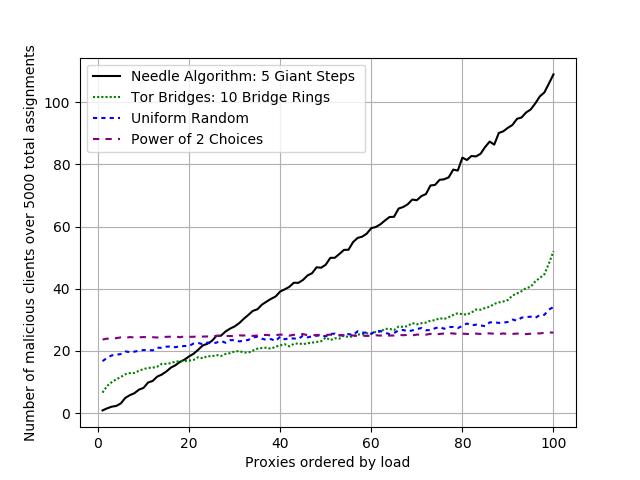
\includegraphics[width=1.0\textwidth]{fig/malicious_comparison_p_50_to_n_100_5000.png}
    \caption{Comparison of Malicious Clients over 5000 assignments with 50\% attackers in the system.}

    \label{fig:malcompare}
\end{figure*}
%%%%%%%%%%%%%%%%%%%%%%%%%%%%%%%%%%%%%%%%%%%%%%%%%%%%%%%%%%%%%%%%%%%%%%

We see from the results of this experiment that the number of malicious clients increases with load in all of the algorithms. The power of 2 choices algorithm has the flattest distribution of malicious clients, meaning that proxies are enumerated the quickest thus creating the highest number of enumerated proxies over all of the algorithms, as we discussed in the enumeration analysis in section \ref{sec:enum}.

When we consider the number of bystanders, we make the assumption that the censor chooses to block the top half of the proxies. These are the proxies that are determined as the most \textit{popular} proxies. Figure \ref{fig:bscompare} shows the total number of bystanders that receive service in each algorithm, assuming that the most heavily loaded $n/2$ proxies are blocked; that is, the rightmost $n/2$ proxies in Figure \ref{fig:malcompare}. The steep slope in the needle's load balancing for the least heavily loaded, leftmost $n/2$ unblocked proxies, allows for a small number of proxies to be preserved, while stacking higher loads onto the remaining proxies. It also serves to distinguish the rightmost proxies as more popular than the others, in a sense serving up these proxies to be blocked as expected collateral damage.

%%%%%%%%%%%%%%%%%%%%%%%%%%%%%%%%%%%%%%%%%%%%%%%%%%%%%%%%%%%%%%%%%%%%%%
\begin{figure*}[h!]
\centering
     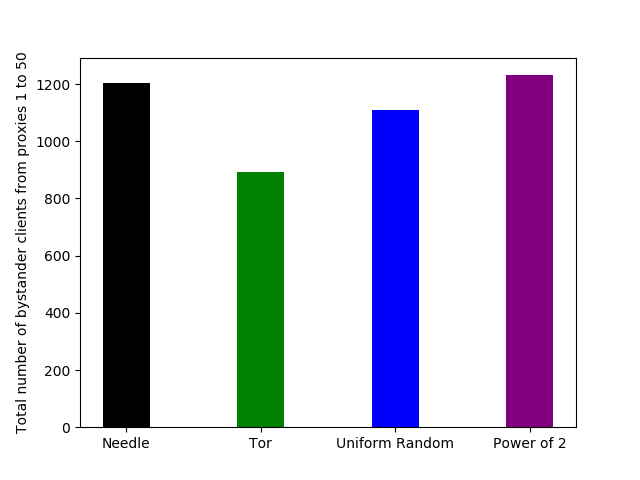
\includegraphics[width=0.8\textwidth]{fig/client_service_p_50_to_n_100_5000.png}
    \caption{Total number of bystander clients in the least popular proxies.}
    \label{fig:bscompare}
\end{figure*}
%%%%%%%%%%%%%%%%%%%%%%%%%%%%%%%%%%%%%%%%%%%%%%%%%%%%%%%%%%%%%%%%%%%%%%

We've shown that by unbalancing the load on the proxies in the needle algorithm, we are still able to service as many or more bystander clients than in the uniform random, power of 2 choices, and Tor's bridgedb mechanism.


\section{Comparison}

We consider enumeration, load balancing, and bystander analyses of the four algorithms in order to contrast their respective trade-offs and suitability under differing system goals. Table \ref{tab:tradeoff} outlines the three metrics that we consider in this thesis. We indicate with checkmarks \ding{51} where the algorithm is well suited, double checkmarks indicate that it is very well suited. A single X mark \ding{55} shows that the algorithm is unsuitable, a double \ding{55}  is used when we consider the algorithm to be completely unusable for a purpose.

The power of 2 choices algorithm provided the best load balancing, and so would be appropriate for systems where this is a concern. However, it is enumerated very quickly.

Uniform random distribution and Tor's \texttt{bridgedb} distribution perform similarly, and so we consider their respective trade-offs in the same vein. They provide a slower enumeration time than the power of 2 choices algorithm due to their uneven load balancing. The number of bystanders is also slightly lower than the other algorithms.

The needle algorithm gives the slowest enumeration of all the algorithms; this attribute is beneficial to allocation of proxies in a distribution system. It is not suitable for systems that require even load balancing. (It is unbalanced to a large degree but not so much that it is unusable.) It services as many bystanders as the power of 2 choices algorithm, but without the drawback of fast enumeration. In the context of proxy distribution under our censorship threat model, we consider this a benefit.

\begin{table}[t]
\begin{tabular}{l*{3}{|c}r}
             & Enumeration & Load Balancing & Bystanders \\
\hline
\hline
power of 2 choices & \ding{55}\ding{55}  & \ding{51}\ding{51} & \ding{51}\ding{51} \\
uniform random            & \ding{55}  & \ding{51} & \ding{55}  \\
Tor's \texttt{bridgedb} & \ding{55}  & \ding{51} & \ding{55}  \\
needle           & \ding{51}\ding{51}  & \ding{55}\ding{55}  & \ding{51}\ding{51}  \\
\end{tabular}
\caption{Comparison chart of the 4 algorithms\label{tab:tradeoff} }
\end{table}